\section{Robots in ASD Interventions}


A recent popular area of research for ASD interventions is robot-based interventions.  This is due to recent advancements in HRI research, as outlined in the previous section, as well as successes shown in studies in using robot in the clinical settings for children with ASD.  Clinical studies of this approach is reviewed by Diehl et al., and the studies have been categorized based on the study purposes \cite{diehl2012clinical}.


\subsection{General Response to Robots}
Several studies have investigated how individuals with ASD interact with robots in general, and have compared it with human counterparts.  Dautenhahn et al. showed that some individuals with ASD prefer interactive robots compared to passive toys \cite{dautenhahn2004towards}.  Robins et al. showed that ASD individuals prefer robot-like characteristics over human-like in social interactions \cite{robins2006does}.  Pierno et al. found that children with ASD respond faster to robotic movement than human movement \cite{pierno2008robotic}.


\subsection{Eliciting Pro-Social Behaviours}
Robins et al. showed that children showed increased social interaction behaviors towards the robot in some areas such as proximity to robot, eye gaze, touch, imitation \cite{robins2005robotic}.  Feil-Seifer et al. suggested that social behaviors of children with ASD increased when the robot is acting contingently to child's actions, as opposed to randomly \cite{feil2009toward}.  Ravindra et al. showed the potential for robot and ASD individuals to share joint attention towards objects \cite{ravindra2009therapeutic}.


\subsection{Modeling, Teaching, or Practicing a Skill and Providing Reinforcements}
Not many studies have been conducted for skill execution training, since most studies have focused on addressing the social aspects of ASD interventions.  One preliminary study by Duquette et al. examined the use of humanoid robot to help children with ASD practice imitation behaviors \cite{duquette2008exploring}.  Positive reinforcements were also given through the robot raising arms and saying ``Happy!'' when the child successfully imitated the robot.  In their study result, children with ASD showed more interest to the robot when the robot is mediating the training session, as compared to their interest during human mediated sessions.  Also, in the robot's presence, fewer repetitive behaviors with their favourite toy were observed.


\subsection{Discussion}
Of particular interest to this thesis is Ravindra et al.'s study \cite{ravindra2009therapeutic}, in which they implemented a detector of object of visual focus of attention.  Using head pose plus eye pose estimations, and mixture of Gaussian modeling of object locations, they were able to detect with 75\% accuracy the object of the child's gaze (i.e. visual focus of attention).  The detector is then used as a feedback to the robot's prompting system for instructing the child to interact with objects through verbal command and gesture prompt (robot points and gazes at the object).


Even though their study's purpose is to train children with ASD with joint attention skills, their study showed the plausibility of utilizing similar techniques for prompting the child to pay attention to or interact with any objects of interest.  Particularly in our thesis, we aim to implement two aspects of their techniques to guide children with ASD through hand-washing:
\begin{itemize}
	\item \textbf{Robot gesture prompt}: point and gaze at an object while instructing the child how to interact with the object.
	\item \textbf{Robot behavior loop}: loop consisting of attention grabber (AG), prompt, reinforcement if instruction successfully followed, loops from AG again if failure (illustrated in Figure \ref{fig:ravindra2009therapeutic}).
\end{itemize}
\begin{figure} [h]
	\centering
	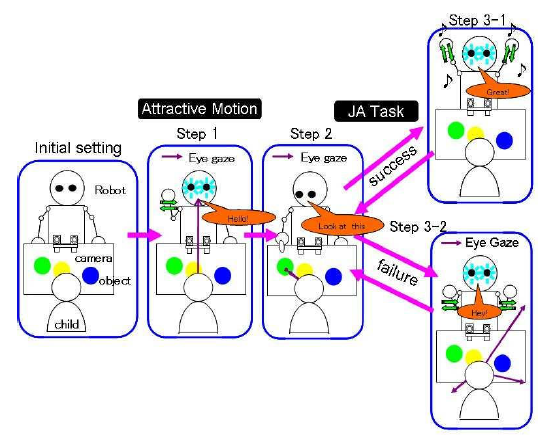
\includegraphics[width=0.6\textwidth]{./img/ravindra2009therapeutic.png}
	\caption{Robot behavior loop used by Ravindra et al. \cite{ravindra2009therapeutic}}
	\label{fig:ravindra2009therapeutic}
\end{figure}

In Diehl et al.'s review, it was pointed out that studies in skill training would benefit from integrating robots into the ABA framework \cite{diehl2012clinical}.  As discussed in Section \ref{sec:DTTDiscussion}, this is what we propose any skill training ATC system should do, similar to COACH.  Thus including a robot into our COACH system would fill this research gap.


In all, from these studies, we see a great potential for increasing the attention and engagement level of the ASD child if we incorporate a humanoid robot into our COACH system.  The robot may serve as an attention grabber as well as a prompting agent.
